\section{Continuum Sensitivity Analysis}
% -.-.-.-.-.-.-.-.-.-.-.-.-.-.-.-.-.-.-.-.-.-.-.-.-.-.-.-.-.-.-.-.-.-.-
\subsection{Formulation}
For a continuous system, the governing equations and boundary conditions are written as

\begin{subequations}\label{eq:C2_continuumGoverningEquation}
\begin{align}
	A(u, t; b) &= 0 \qquad \qquad \text{on } \Omega \\
	B(u, t; b) &= g(x, t; b) \quad \text{on } \Gamma
\end{align}	
\end{subequations}

where $u$ is the response variable, i.e. displacement or pressure, $t$ is time, $x$ is the spatial coordinate, and $b$ is the design variable that can be used to control the solution. $A$ and $B$ are continuum functions that define the governing equations and boundary conditions respectively. It should be noted that the governing equation is written in the residual form where its value needs to be equal to zero when $u$ is the solution at time $t$. $g$ is the value of the boundary condition of the defined system. To calculate the sensitivity of response, it is required to calculate the total derivative of Equation \eqref{eq:C2_continuumGoverningEquation}. This is done by calculating the local sensitivity of the governing equation followed by converting the local sensitivities to their total form using Equation \eqref{eq:C2_totalSensitivityDef}.

The governing equation and the boundary condition of \eqref{eq:C2_continuumGoverningEquation} are differentiated as follows

\begin{subequations}\label{eq:C2_continuumSensitivityFormulation}
\begin{align}
	A(u', t; b) + A'(u, t; b) &= 0 \qquad \qquad \text{on } \Omega \\
	B(\dot{u}, t; b) + \dot{B}(u, t; b) &= \dot{g}(x, t; b) \quad \text{on } \Gamma
\end{align}	
\end{subequations}

where $(\text{ })'$ and $\dot{(\text{ })}$ are local and total derivative which are defined as follows

\begin{subequations}
\begin{align*}
	(\text{ })' &= \frac{\partial (\text{ })}{\partial b} \\
	\dot{(\text{ })} &= \frac{D (\text{ })}{D b}
\end{align*}
\end{subequations}

It should be noted that the governing equations are differentiated in the local form and the boundary conditions are differentiated in the total form. Local differentiation of the governing equations enables us to treat the solver non-intrusively \cite{cross2014local}. However, in order to capture the effect of shape change, the boundary conditions need to be differentiated in the total form. The boundary condition definition is further simplified by assuming linearly. This is a valid assumption for many practical cases such as structural analysis or computational fluid dynamics. The boundary conditions are usually in the form of known gradient or values, i.e. outflow and free-slip wall for CFD and predefined displacement/force for structural analysis. It should be noted that this assumption is not valid for problems such as contacts. The boundary condition is written as

\begin{align}\label{eq:C2_linearSAboundaryCondtions}
\begin{split}
	B(\dot{u}, t; b) &= \dot{g}(x, t; b) \Rightarrow \\
	B(u', t; b) &= \dot{g}(x, t; b) - B(\frac{\partial u}{\partial x} \cdot \frac{\partial x}{\partial b}, t; b)
\end{split}
\end{align}

To study the differentiated governing equation of Equation \eqref{eq:C2_continuumSensitivityFormulation}, we will assume two situations: i) linear analysis, ii) nonlinear analysis.

For the linear analysis, the governing  of \eqref{eq:C2_continuumSensitivityFormulation} is written as

\begin{equation}\label{eq:C2_linearSAgoverningEquation}
	A(u', t; b) = 0 
\end{equation}

This is valid since for the linear case, the differential operators of the governing equation do not depend on the response variable, $u$. To explain this concept, we look at the transient heat conduction in 1D domain. The governing equations are defined as

\begin{equation}\label{eq:C2_transientHeatCondtionGE}
	\frac{\partial^2 T}{\partial x^2} = \frac{1}{\alpha} \frac{\partial T}{\partial t}
\end{equation}

where $T$ is the temperature, $x$ is spatial coordinate, $t$ is time, and $\alpha$ is is the thermal diffusivity ($k/\rho c_p$). This equation can be differentiated with respect to a design variable $b$ as shown in the following equation.

\begin{equation*}
	\frac{\partial}{\partial b}
	\left( \frac{\partial^2 T}{\partial x^2}\right) = 
	\frac{\partial}{\partial b}
	\left( \frac{1}{\alpha} \frac{\partial T}{\partial t}\right)
\end{equation*}

Due to linearity of the differential operators we can change the order of differentiation as follows

\begin{equation}\label{eq:C2_transientHeatCondtionSA}
	\frac{\partial^2}{\partial x^2}
	\left( \frac{\partial T}{\partial b} \right) = 
	\frac{1}{\alpha} \frac{\partial}{\partial t}
	\left( \frac{\partial T}{\partial b}\right)
\end{equation}

By comparing Equations \eqref{eq:C2_transientHeatCondtionGE} and \eqref{eq:C2_transientHeatCondtionSA} we can see that the differential operators, $\partial^2 /\partial x^2$, and $\partial /\partial t$ remain unchanged. Therefore, same solver can be used for solving this system of governing equations and for the sensitivity variable, $\partial T/\partial b$.

For nonlinear problems, the differential operators are functions of response variable as well. For example, the incompressible Euler's equation for a 2D flow is derived as

\begin{subequations}\label{eq:C2_eulerEquations}
\begin{gather}
	\frac{\partial u}{\partial t} +
	u \frac{\partial u}{\partial x} + v \frac{\partial u}{\partial y} +
	\frac{\partial p}{\partial x} = 0 
	\\
	\frac{\partial v}{\partial t} +
	u \frac{\partial v}{\partial x} + v \frac{\partial v}{\partial y} +
	\frac{\partial p}{\partial y} = 0
\end{gather}
\end{subequations}

where $u$ and $v$ are the velocity components in $x$ and $y$ directions respectively. $p$ is pressure, $t$ is time, $x$ and $y$ are spatial coordinates. We can rewrite Equation \eqref{eq:C2_eulerEquations} in terms of differential operators too.

\begin{subequations}
\begin{gather*}
	\mathcal{T} u +
	\mathcal{C} u +
	\mathcal{G}_x p = 0 
	\\
	\mathcal{T} v +
	\mathcal{C} v +
	\mathcal{G}_y p = 0 
\end{gather*}
\end{subequations}

where $\mathcal{T}$ is the time derivative operator ($\partial /\partial t$), $\mathcal{C}$, is the convective operator as shown in Equation \eqref{eq:C2_convectiveOperator}.

\begin{equation}\label{eq:C2_convectiveOperator}
	\mathcal{C} = u \frac{\partial}{\partial x} + v \frac{\partial}{\partial y}
\end{equation}

$\mathcal{G}_x$ and $\mathcal{G}_y$ are gradient operators in $x$ and $y$ respectively ($\partial /\partial x$ and $\partial /\partial y$). The gradient and time derivative operators are linear, therefore they can be treated as shown in the previous paragraphs. On the other hand, the convective operator is nonlinear and it should be differentiated with response variables as well. As a result, the sensitivity equations can be written in the operator form as

\begin{subequations}\label{eq:C2_eulerEquationsSA}
\begin{gather}
	\mathcal{T} u' +
	\mathcal{C}' u + \mathcal{C} u' +
	\mathcal{G}_x p' = 0 
	\\
	\mathcal{T} v' +
	\mathcal{C}' v + \mathcal{C} v' +
	\mathcal{G}_y p' = 0 
\end{gather}
\end{subequations}

where

\begin{equation*}
	\mathcal{C}' = u' \frac{\partial}{\partial x} + v' \frac{\partial}{\partial y}
\end{equation*}

Several interesting properties of CSA can be explained using Equation \eqref{eq:C2_eulerEquationsSA}. First of all, although the original Euler equation is nonlinear due to multiplication of response variables and their derivatives ($u$ and $\partial u/\partial x$), the resulting sensitivity equation is linear. This means that the sensitivity equations are easier to solve both in terms of algorithms and simulation time compared to the original equations. The challenging expression that needs to be calculated in Equation \eqref{eq:C2_eulerEquationsSA} is the convective term derivative.

The first step in solving the sensitivity equations is to get the solution of the governing equations. This enables us to calculate the convective operator, $\mathcal{C}$, at each step of sensitivity solution based on the analysis data. $\mathcal{C}'$ is also calculated at each step of the solution of sensitivity equations based on the solution as previous time step. For a simple predictor–corrector method used to solving the original governing equations, this can be written as follows for sensitivity equation in $x$ direction.

\begin{align*}
	\bar{u}' &= u'(i) - 
	\Delta t \left[ \mathcal{C}'(i) u(i) + \mathcal{C}(i) u'(i) + \mathcal{G} p'(i) \right]
	\qquad \qquad \qquad \qquad \qquad \qquad \qquad \text{: predictor}
	\\
	u'(i+1) &= u'(i) + \frac{\Delta t}{2} - 
	\left[ \mathcal{C}'(i) u(i) + \mathcal{C}(i) u'(i) + \mathcal{G} p'(i) + \bar{\mathcal{C}}(i) u(i) + \mathcal{C}(i) \bar{u} + \mathcal{G} p'(i)\right]
	\quad \text{: corrector}
\end{align*}

In above equations, $\bar{\mathcal{C}}$ in the convective operator evaluated using $\bar{u}$. It should be noted that in order to generate the operator we do not need to know the details of how it has been put together. We only supply the required material for generating the convective operator and the black-box solver will generate it for us. This input is response variable when solving the governing equation, and is the sensitivity of response variable for sensitivity analysis. Therefore, the solver can still be considered as a black box that we do not modify.

% -.-.-.-.-.-.-.-.-.-.-.-.-.-.-.-.-.-.-.-.-.-.-.-.-.-.-.-.-.-.-.-.-.-.-.-.-.-.-.-.-.-.-.-.-.-
\subsection{Implementation for heat transfer problem}
In this section, the continuum sensitivity formulation is used for calculating the sensitivity of temperature with respect to length of a 1D domain. The domain is defined in Figure \ref{fig:C2_benchmarkCase} with the temperature in the domain is governed by Equation \eqref{eq:C2_laplaceEquation}. The boundary conditions are defined as $T_0$ at $x=0$ and $T_L$ at $x=L$.

To get the sensitivity equations, governing equations are differentiated in the local form and boundary conditions are differentiated in total form as shown in Equation \eqref{eq:C2_differentiatedLaplaceEquation}.

\begin{equation}\label{eq:C2_differentiatedLaplaceEquation}
	\frac{\partial}{\partial L}
	\left( \frac{\partial^2 T}{\partial x^2} = 0 \right)
\end{equation}

Since the differential operator is linear, the order of differentiations is changed. This will give us the following equation for the sensitivity calculation.

\begin{equation}\label{eq:C2_laplaceSAequation}
	\frac{\partial^2}{\partial x^2} \left( \frac{\partial T}{\partial L} \right) = 0
\end{equation}

The boundary conditions for this problem are written as follows to be consistent with the general formulation of the boundary conditions. 

\begin{equation}\label{eq:C2_laplaceEquationBoundaryCondition}
\begin{cases}
	\mathcal{B}T = T_0 \qquad \text{at x = 0} \\
	\mathcal{B}T = T_L \qquad \text{at x = L}
\end{cases}
\end{equation}

where $\mathcal{B}$ is the operator acting on the boundary. For this problem, it is equal to $1$. Equation \eqref{eq:C2_laplaceEquationBoundaryCondition} is differentiated in the total form since the boundaries are moving. This results in

\begin{equation}
\begin{cases}
	\dot{\mathcal{B}} T + \mathcal{B} \dot{T} = \dot{T}_0 \qquad \text{at x = 0} \\
	\dot{\mathcal{B}} T + \mathcal{B} \dot{T} = \dot{T}_L \qquad \text{at x = L}
\end{cases}
\end{equation}

$\mathcal{B}$ and $\dot{T}_0$ are constants and have zero derivative. $\dot{T}$ is written in terms of the local derivative and convective terms using the chain rule. This results in the following definition for the sensitivity equation boundary conditions.

\begin{equation*}
\begin{cases}
	\dfrac{\partial T}{\partial b} = -\dfrac{\partial T}{\partial x} \dfrac{\partial x}{\partial b} \qquad \text{at x = 0}
	\\
	\dfrac{\partial T}{\partial b} = -\dfrac{\partial T}{\partial x} \dfrac{\partial x}{\partial b} \qquad \text{at x = L}
\end{cases}
\end{equation*}

To calculate the mesh sensitivity at the boundary, the dependency of spatial variable, $x$, and the shape of the domain, $L$, need to be known. For the 1D domain, this is defined as follows

\begin{equation*}
	x = \alpha L
\end{equation*}

This means that every location in the domain can be defined using a nondimensional variable, $\alpha$, times the total length of the domain. Using this formulation, the sensitivity of spatial coordinate, $x$, with respect to the length of the domain is defined as

\begin{equation*}
	\frac{\partial x}{\partial L} = \alpha \quad \text{where } \quad \alpha = \frac{x}{L}
\end{equation*}

By using this relation, the boundary conditions can be written as

\begin{equation*}
\begin{cases}
	\mathcal{B} \dfrac{\partial T}{\partial b} = -\dfrac{\partial T}{\partial x} \dfrac{x}{L} \qquad \text{at x = 0}
	\\
	\mathcal{B} \dfrac{\partial T}{\partial b} = -\dfrac{\partial T}{\partial x} \dfrac{x}{L} \qquad \text{at x = L}
\end{cases}
\end{equation*}

This can be further simplified by substituting $x$ in the definition of boundary conditions. We also substitute $\mathcal{B}$ as 1.

\begin{equation}\label{eq:C2_laplaceSAboundaryCondition}
\begin{cases}
	\dfrac{\partial T}{\partial b} = 0 \qquad \text{at x = 0}
	\\
	\dfrac{\partial T}{\partial b} = -\dfrac{\partial T}{\partial x} \qquad \text{at x = L}
\end{cases}
\end{equation}

The last thing to be noted is the spatial derivative of response variable at the boundaries, $\partial T/\partial x$. This term appears due to the boundary movement with change in shape design variable when using the chain rule. This term is calculated from the analysis results by using the same technique used for discretizing the governing equations. For this problem, the finite difference method is used to calculate this derivative from the analysis results.

The governing equation of \eqref{eq:C2_laplaceSAequation} with boundary condition \eqref{eq:C2_laplaceSAboundaryCondition} is solved using the same solver that we used for solving the original governing equation since these two are effectively having the same form. The comparison between the original governing equation and the sensitivity equation is shown in Table \ref{table:C2_comparisonBetweenGEandSA}.

\begin{center}
\begin{table}[h]
\begin{tabular}{| c | c | c | c | c |}
	\hline
	Analysis Type & Equation & Unknowns & Discretized form & Discretization method \\ \hline \hline
	Governing equation & $\partial^2 T/\partial x^2$ & $T$ & $[K][T] = [F_{BC}]$ & Central difference \\ \hline
	Sensitivity equation & $\partial^2 T'/\partial x^2$ & $T'$ & $[K][T'] = [F'_{BC}]$ & Central difference \\ \hline
\end{tabular}
\caption{Comparison between the governing and sensitivity equations.}
\label{table:C2_comparisonBetweenGEandSA}
\end{table}
\end{center}

The continuum sensitivity analysis (CSA) result is verified using the analytical solution of Equation \eqref{eq:C2_benchmarkCaseAnalyticalSolution} as shown in Figure \ref{fig:C2_comparisonBetweenCSAandAnalytical}. Different number of discretization nodes are used for the comparison between the results. For the qualitative comparison between the results, the NRMSD as defined in Equation \eqref{eq:C2_NRMSD} is used. As shown if Figure \ref{fig:C2_comparisonBetweenCSAandAnalytical} and Table \ref{table:C2_CSA_NRMSD}, the two results match perfectly.

\begin{figure}[H]
	\centering
	\subfigure[$n = 11$]
	{
	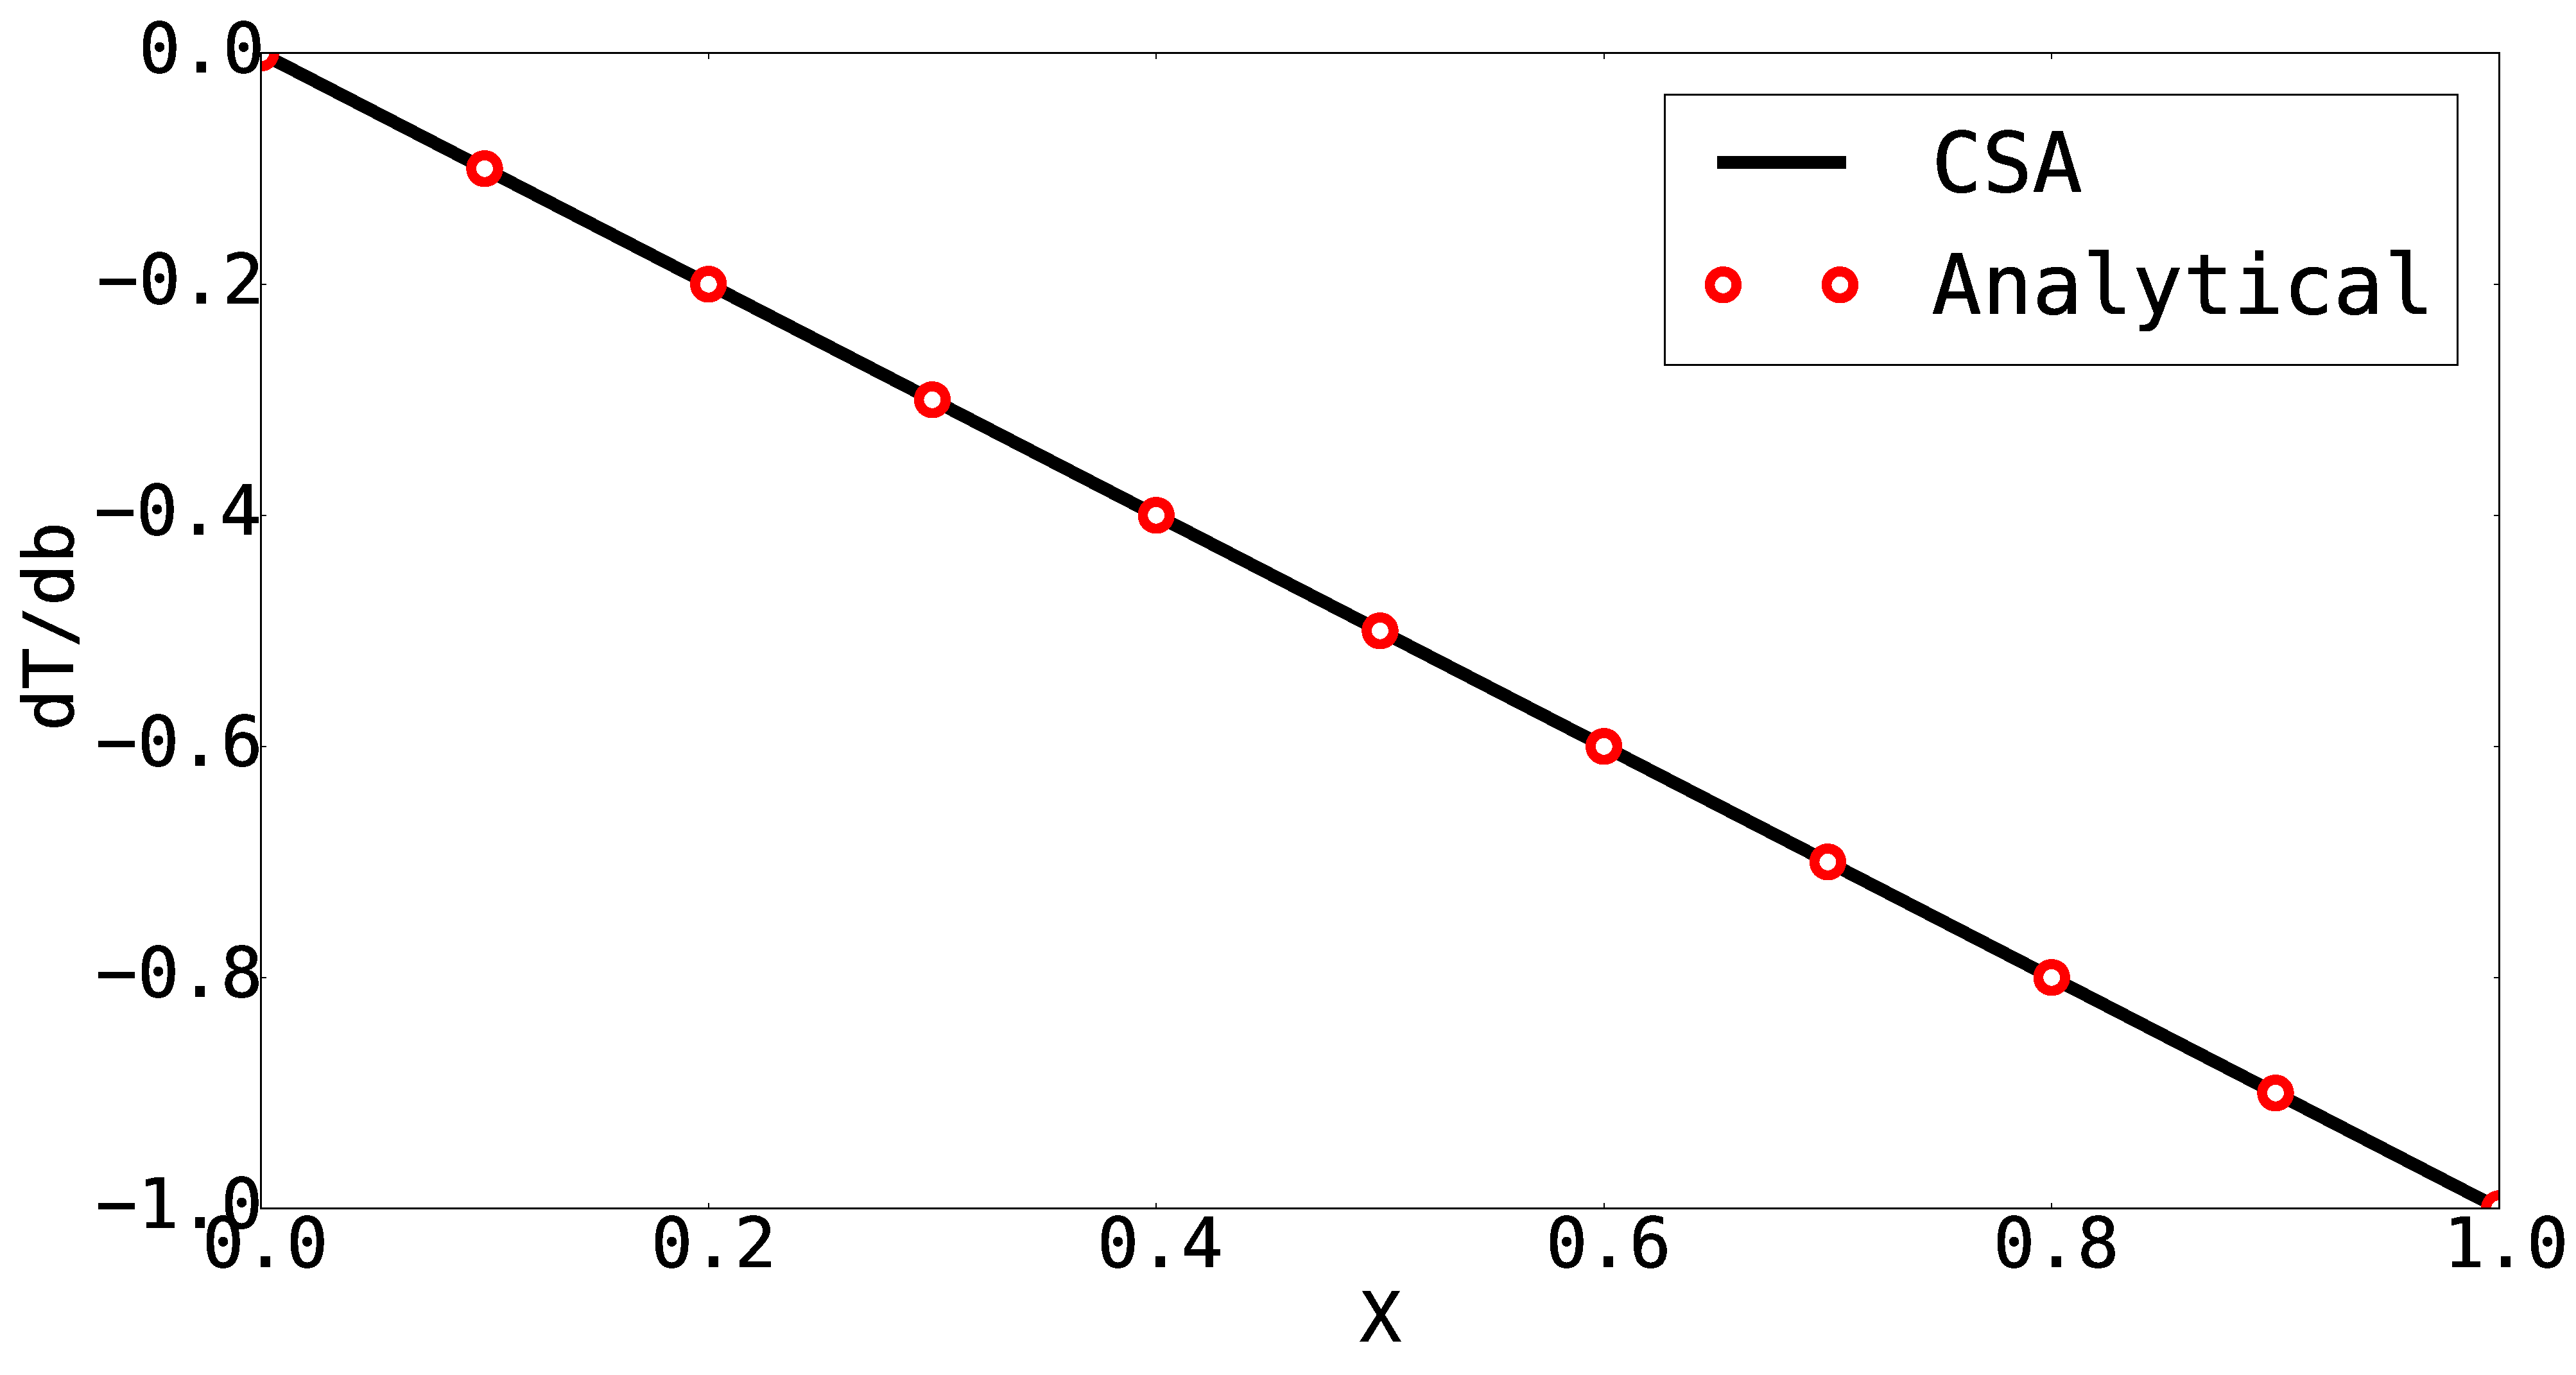
\includegraphics[width=7.0cm]{Chapter_2/figure/CSA_n11.eps}
	}
	\quad
	\subfigure[$n = 41$]
	{
	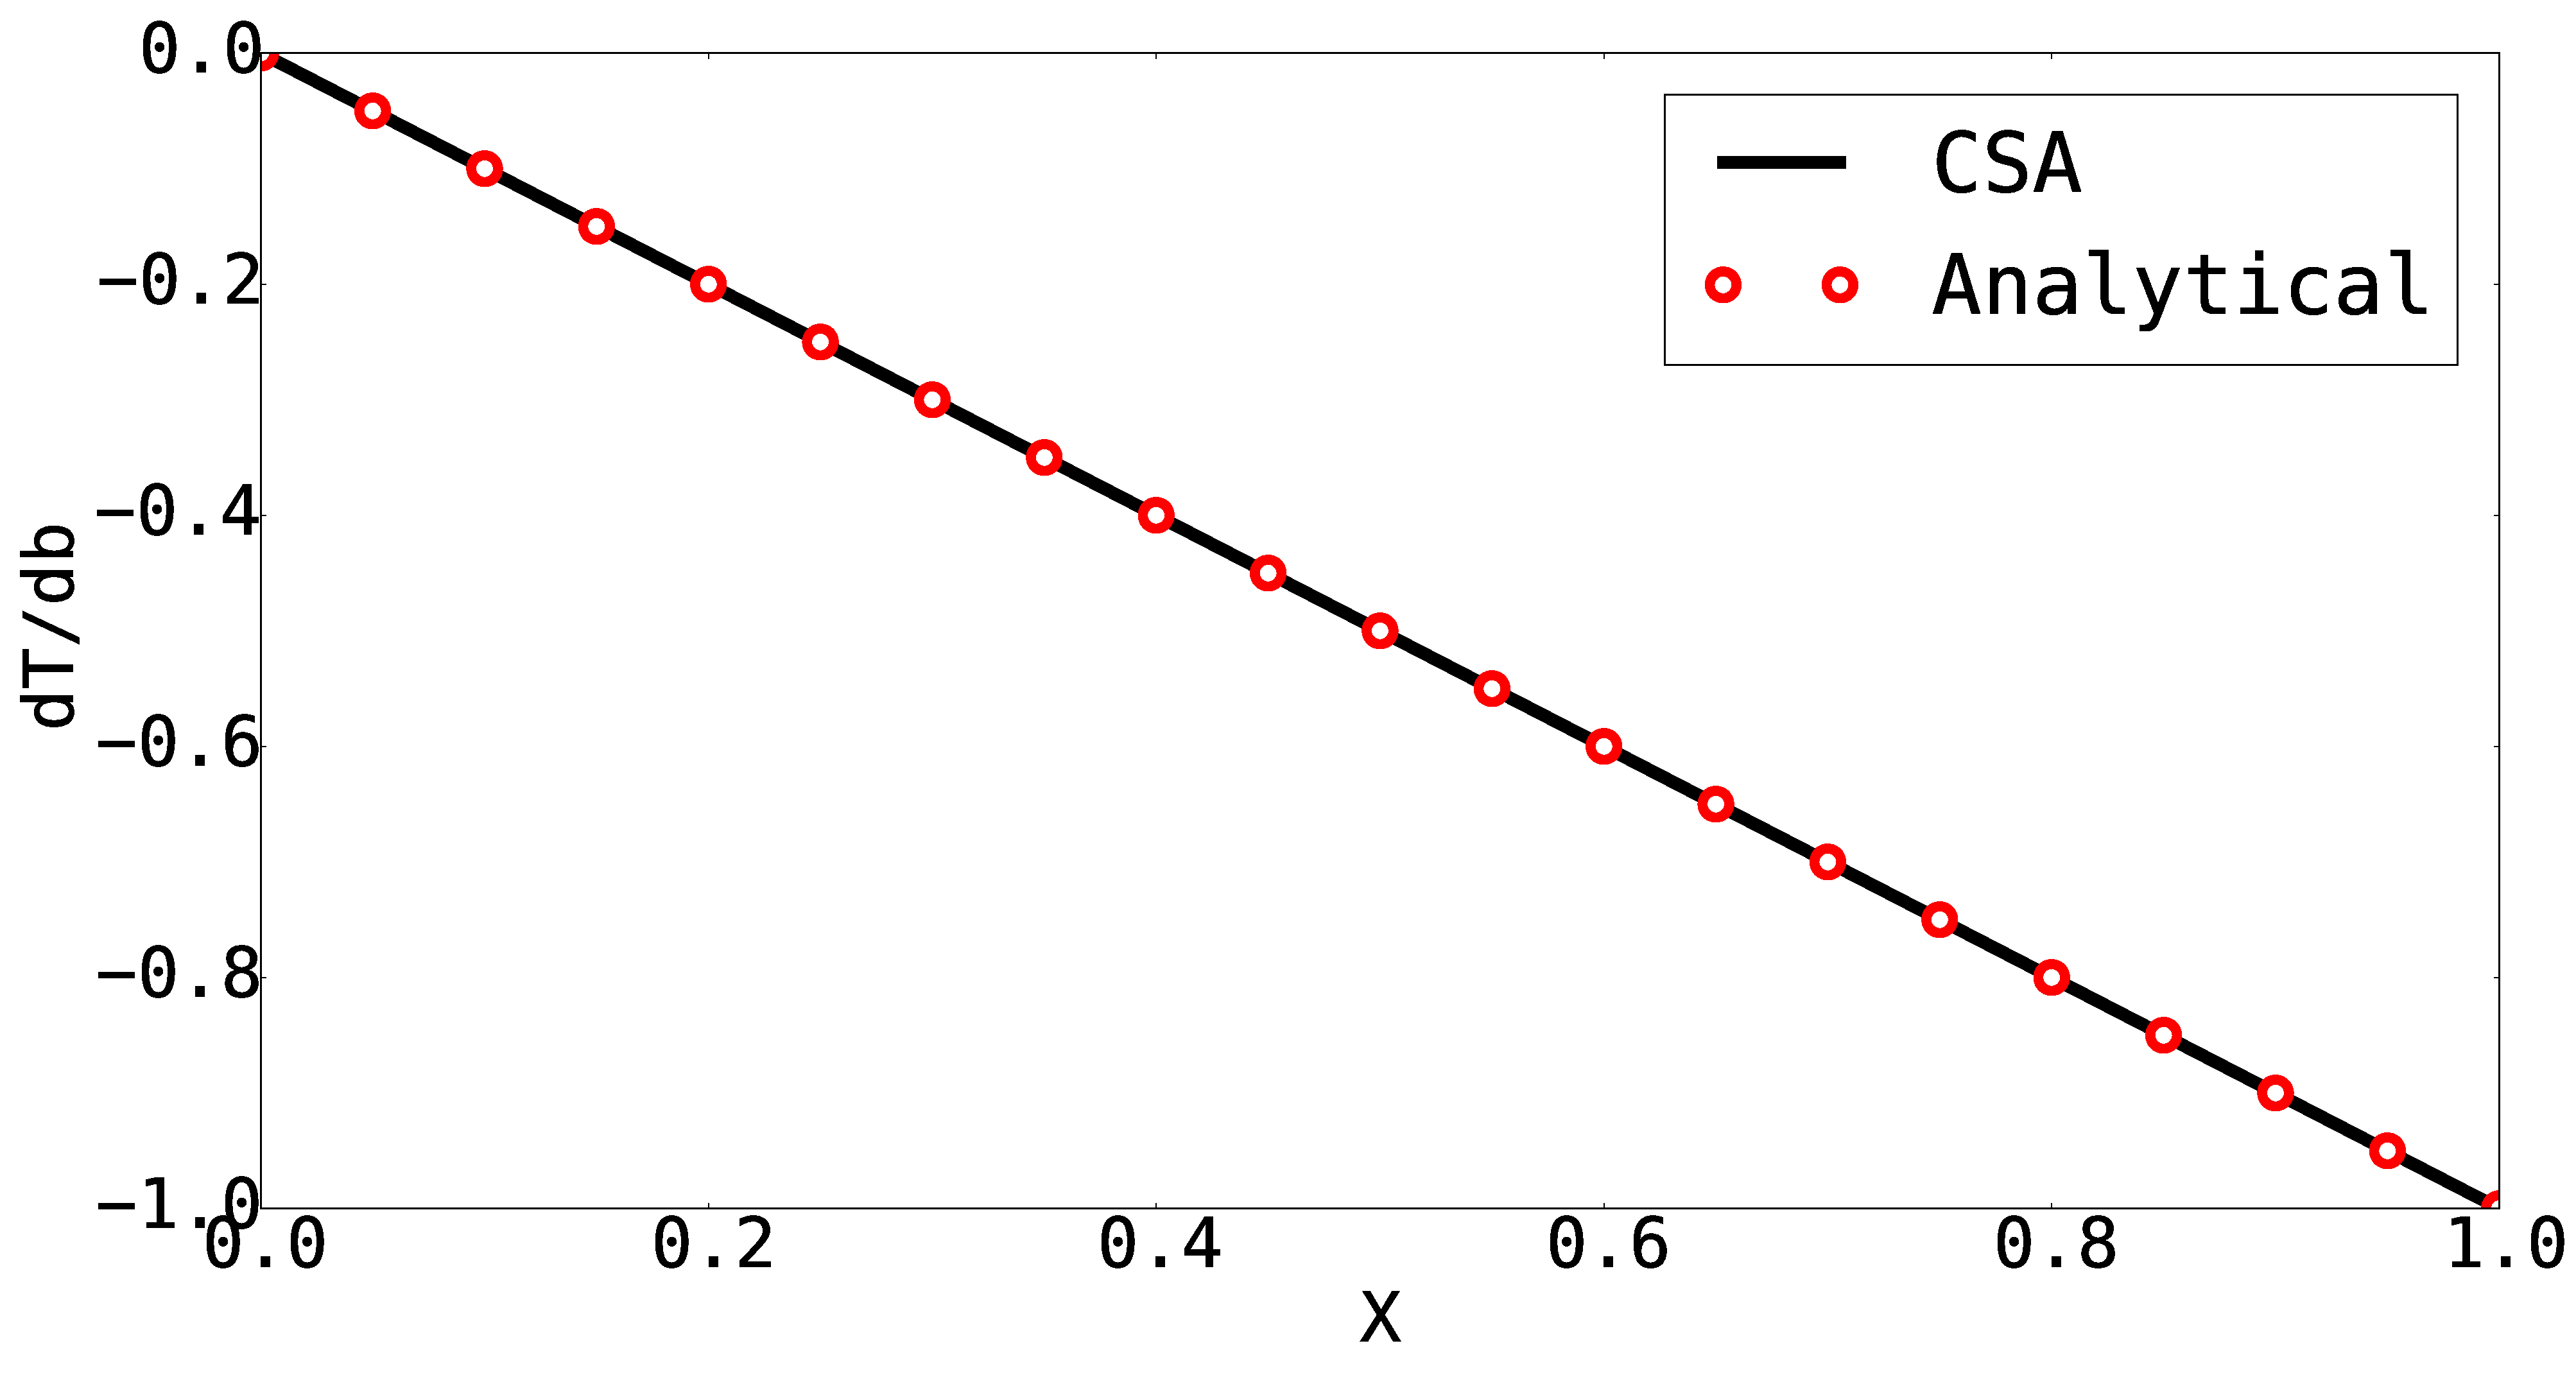
\includegraphics[width=7.0cm]{Chapter_2/figure/CSA_n41.eps}
	}
	\\
	\subfigure[$n = 81$]
	{
	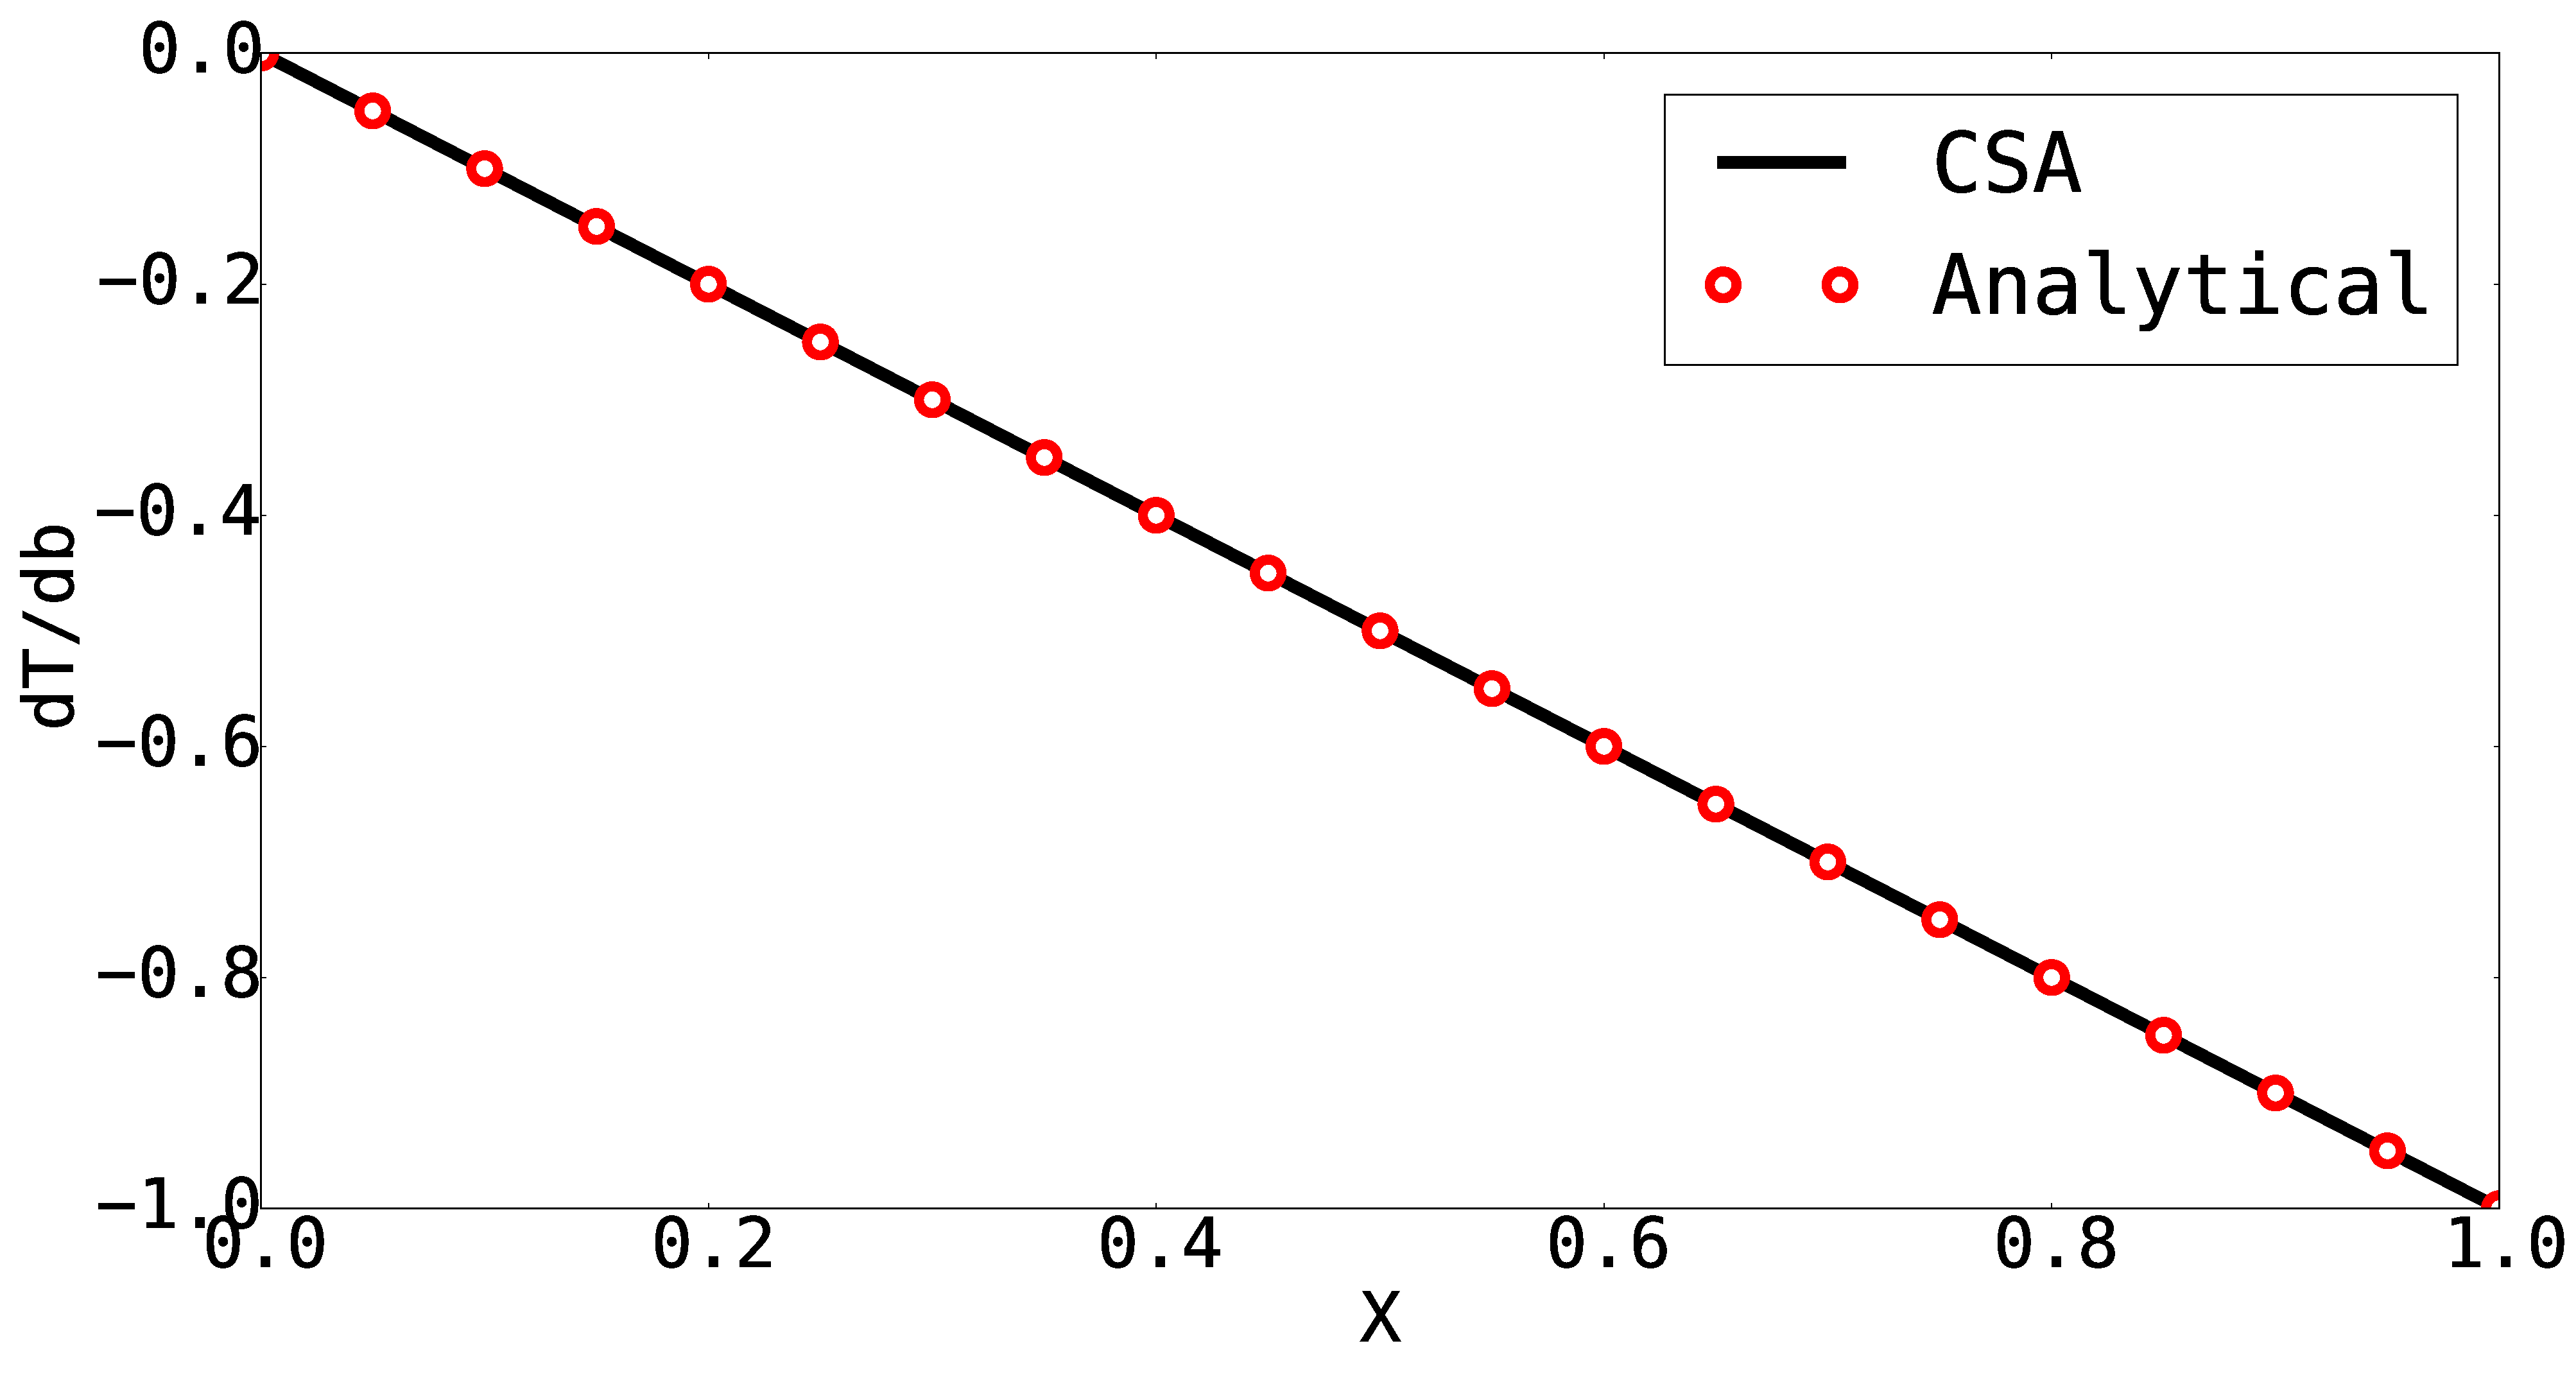
\includegraphics[width=7.0cm]{Chapter_2/figure/CSA_n81.eps}
	}
	\quad
	\subfigure[$n = 161$]
	{
	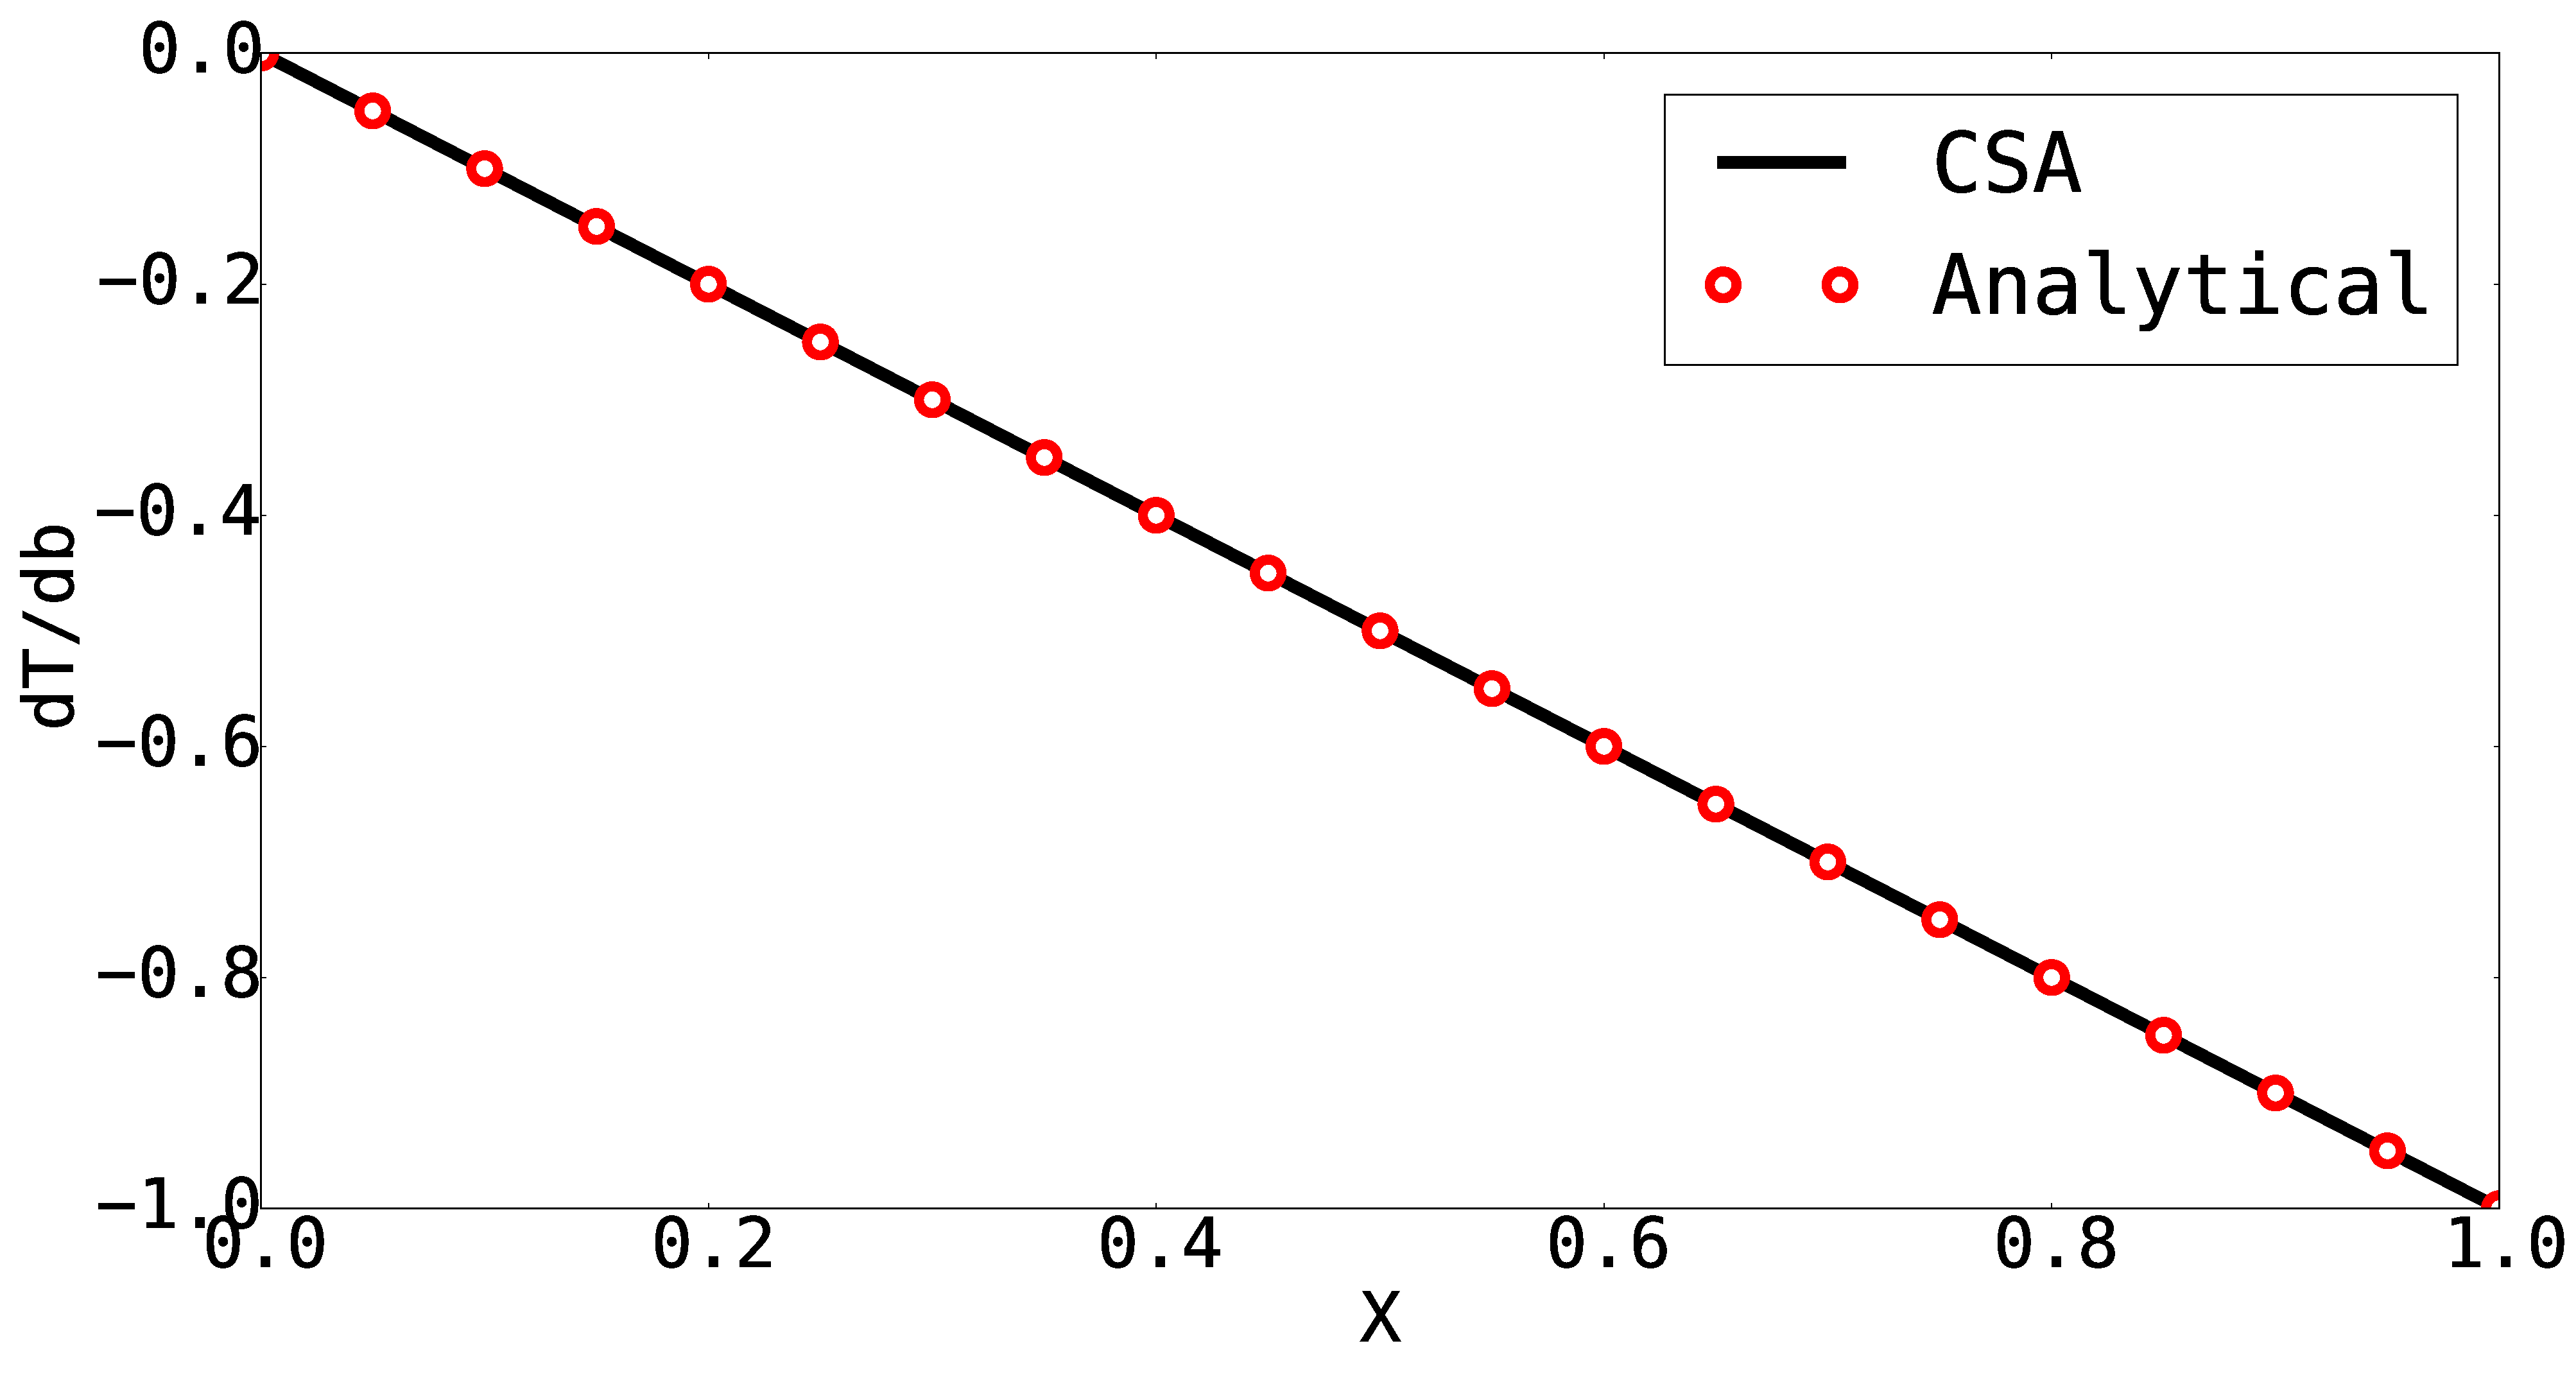
\includegraphics[width=7.0cm]{Chapter_2/figure/CSA_n161.eps}
	}
	\caption{Comparison between continuum sensitivity analysis and analytical results for different number of nodes.}
	\label{fig:C2_comparisonBetweenCSAandAnalytical}
\end{figure}

\begin{table}[H]
\centering
\begin{tabular}{| c | c |}
	\hline
	Number of nodes & NRMSD \\ \hline \hline
	11 & $6.96 \times 10^{-17}$ \\ \hline
	41 & $2.02 \times 10^{-15}$ \\ \hline
	81 & $1.43 \times 10^{-15}$ \\ \hline
	161 & $2.77 \times 10^{-15}$ \\ \hline
\end{tabular}
\caption{RMSE value for different number of nodes.}
\label{table:C2_CSA_NRMSD}
\end{table}

It should be noted that the sensitivity equations are derived and solved in the local form. This does not include the effect of nodes moving in the computational domain. If the analysis requires the sensitivity at the material points, an additional step is required to convert the local sensitivities to their total form using the chain rule as shown in the following equation.

\begin{equation*}
	\frac{DT}{Db} = \frac{\partial T}{\partial b} + \frac{\partial T}{\partial x} \cdot \frac{\partial x}{\partial b}
\end{equation*}

This will add an extra cost to the simulation due to additional step for calculating $\partial x/\partial b$. The reason this step exists is due to movement of computational nodes due to change in shape. Therefore, if the computational nodes can be fixed, the $\partial x/\partial b$ term will be equal to zero. We are proposing to achieve this using a non-body conformal technique such as immersed boundary method. This will be explained in the next chapter in more details.

% -.-.-.-.-.-.-.-.-.-.-.-.-.-.-.-.-.-.-.-.-.-.-.-.-.-.-.-.-.-.-.-.-.-.-.-.-.-.-.-.-.-.-.-.-
\subsection{Implementation for solid mechanics problem}
To derive the continuum sensitivity equations, the governing equation of \eqref{eq:C2_axialBarGE} is differentiated with respect to the design variable, $L$, as shown in Equation \eqref{eq:C2_axialBarContinuumSensitivityEquation}.

\begin{equation}\label{eq:C2_axialBarContinuumSensitivityEquation}
	\frac{\partial^2}{\partial x^2} \left( \frac{\partial u}{\partial L} \right) - 
	\frac{\pi x}{L^2} \cos \left( \frac{\pi x}{L} \right) = 0
\end{equation}

The boundary conditions are calculated by differentiating the boundary conditions defined in Equation \eqref{eq:C2_axialBarBC}. It should be noted that the boundary conditions are differentiated in total form.

\begin{equation}\label{eq:C2_axialBarContinuumSensitivityBoundaryConditions}
	\begin{cases}
	\dfrac{\partial}{\partial x} \left( \dfrac{\partial u}{\partial L} \right) \bigg|_{x = 0} = 
	\dfrac{\partial }{\partial L} \left( \dfrac{1}{\pi} \right) = 0
	\\
	\dfrac{\partial}{\partial x} \left( \dfrac{\partial u}{\partial L} \right) \bigg|_{x = L} = 
	\left\{
	K \left[ \dfrac{\partial u}{\partial L} + \dfrac{\partial u}{\partial x} \dfrac{\partial x}{\partial L} \right] - 
	\dfrac{\partial^2 u}{\partial x^2} \dfrac{\partial x}{\partial L}
	\right\} \bigg|_{x = L}
	\end{cases}
\end{equation}

For this problem, the spatial coordinate $x$ is defined as $x = \zeta L$ where $\zeta = x / L$. Therefore, the design velocity $\partial x/\partial L$ at $x = L$ is equal to one. Solving the governing equation \eqref{eq:C2_axialBarContinuumSensitivityEquation} along with boundary conditions \eqref{eq:C2_axialBarContinuumSensitivityBoundaryConditions} leads to the sensitivity values of displacement in the domain, $\partial u/\partial L$. Comparing the sensitivity equation and boundary conditions \eqref{eq:C2_axialBarContinuumSensitivityEquation} and \eqref{eq:C2_axialBarContinuumSensitivityBoundaryConditions} to the governing equation and its corresponding boundary conditions of \eqref{eq:C2_axialBarGE} and \eqref{eq:C2_axialBarBC}, it is safe to say that these equations are the same. Only the boundary conditions are different between these two system of equations. Therefore, the same numerical solver that was used for solving the governing equation can be used to solve the sensitivity equations without any modifications. The only change would be in the values of the boundary conditions. However, change in the boundary conditions does not change the structure of the black box solver.

To calculate the sensitivities, the governing equation and boundary conditions of \eqref{eq:C2_axialBarContinuumSensitivityEquation} and \eqref{eq:C2_axialBarContinuumSensitivityBoundaryConditions} are discretized using the finite element method as discussed through equations \eqref{eq:C2_stiffnessMatrixOfBar} and \eqref{eq:C2_discretizedBarEquation}. It should be noted that $[K]$ and $[K_s]$ are the same matrices that used in Equation \eqref{eq:C2_stiffnessMatrixOfBar}, $[F_p]$ is equal to zero, and $F_d = -\dfrac{\pi x}{L^2} \cos \left( \dfrac{\pi x}{L} \right)$. For verification, the results for the sensitivity analysis are compared with the analytical results of sensitivity as defined by Equation \eqref{eq:C2_axialBarSensitivitySolution}. We used the NRMSE metric to compare the two different results as defined in Equation \eqref{eq:C2_NRMSE_beam}. The comparison of the results are shown in Figure \ref{fig:C2_continuumSensitivityResults}. As shown here, the results for both discrete and continuum sensitivity analysis converge with the same rate.

\begin{figure}[h]
	\centering
	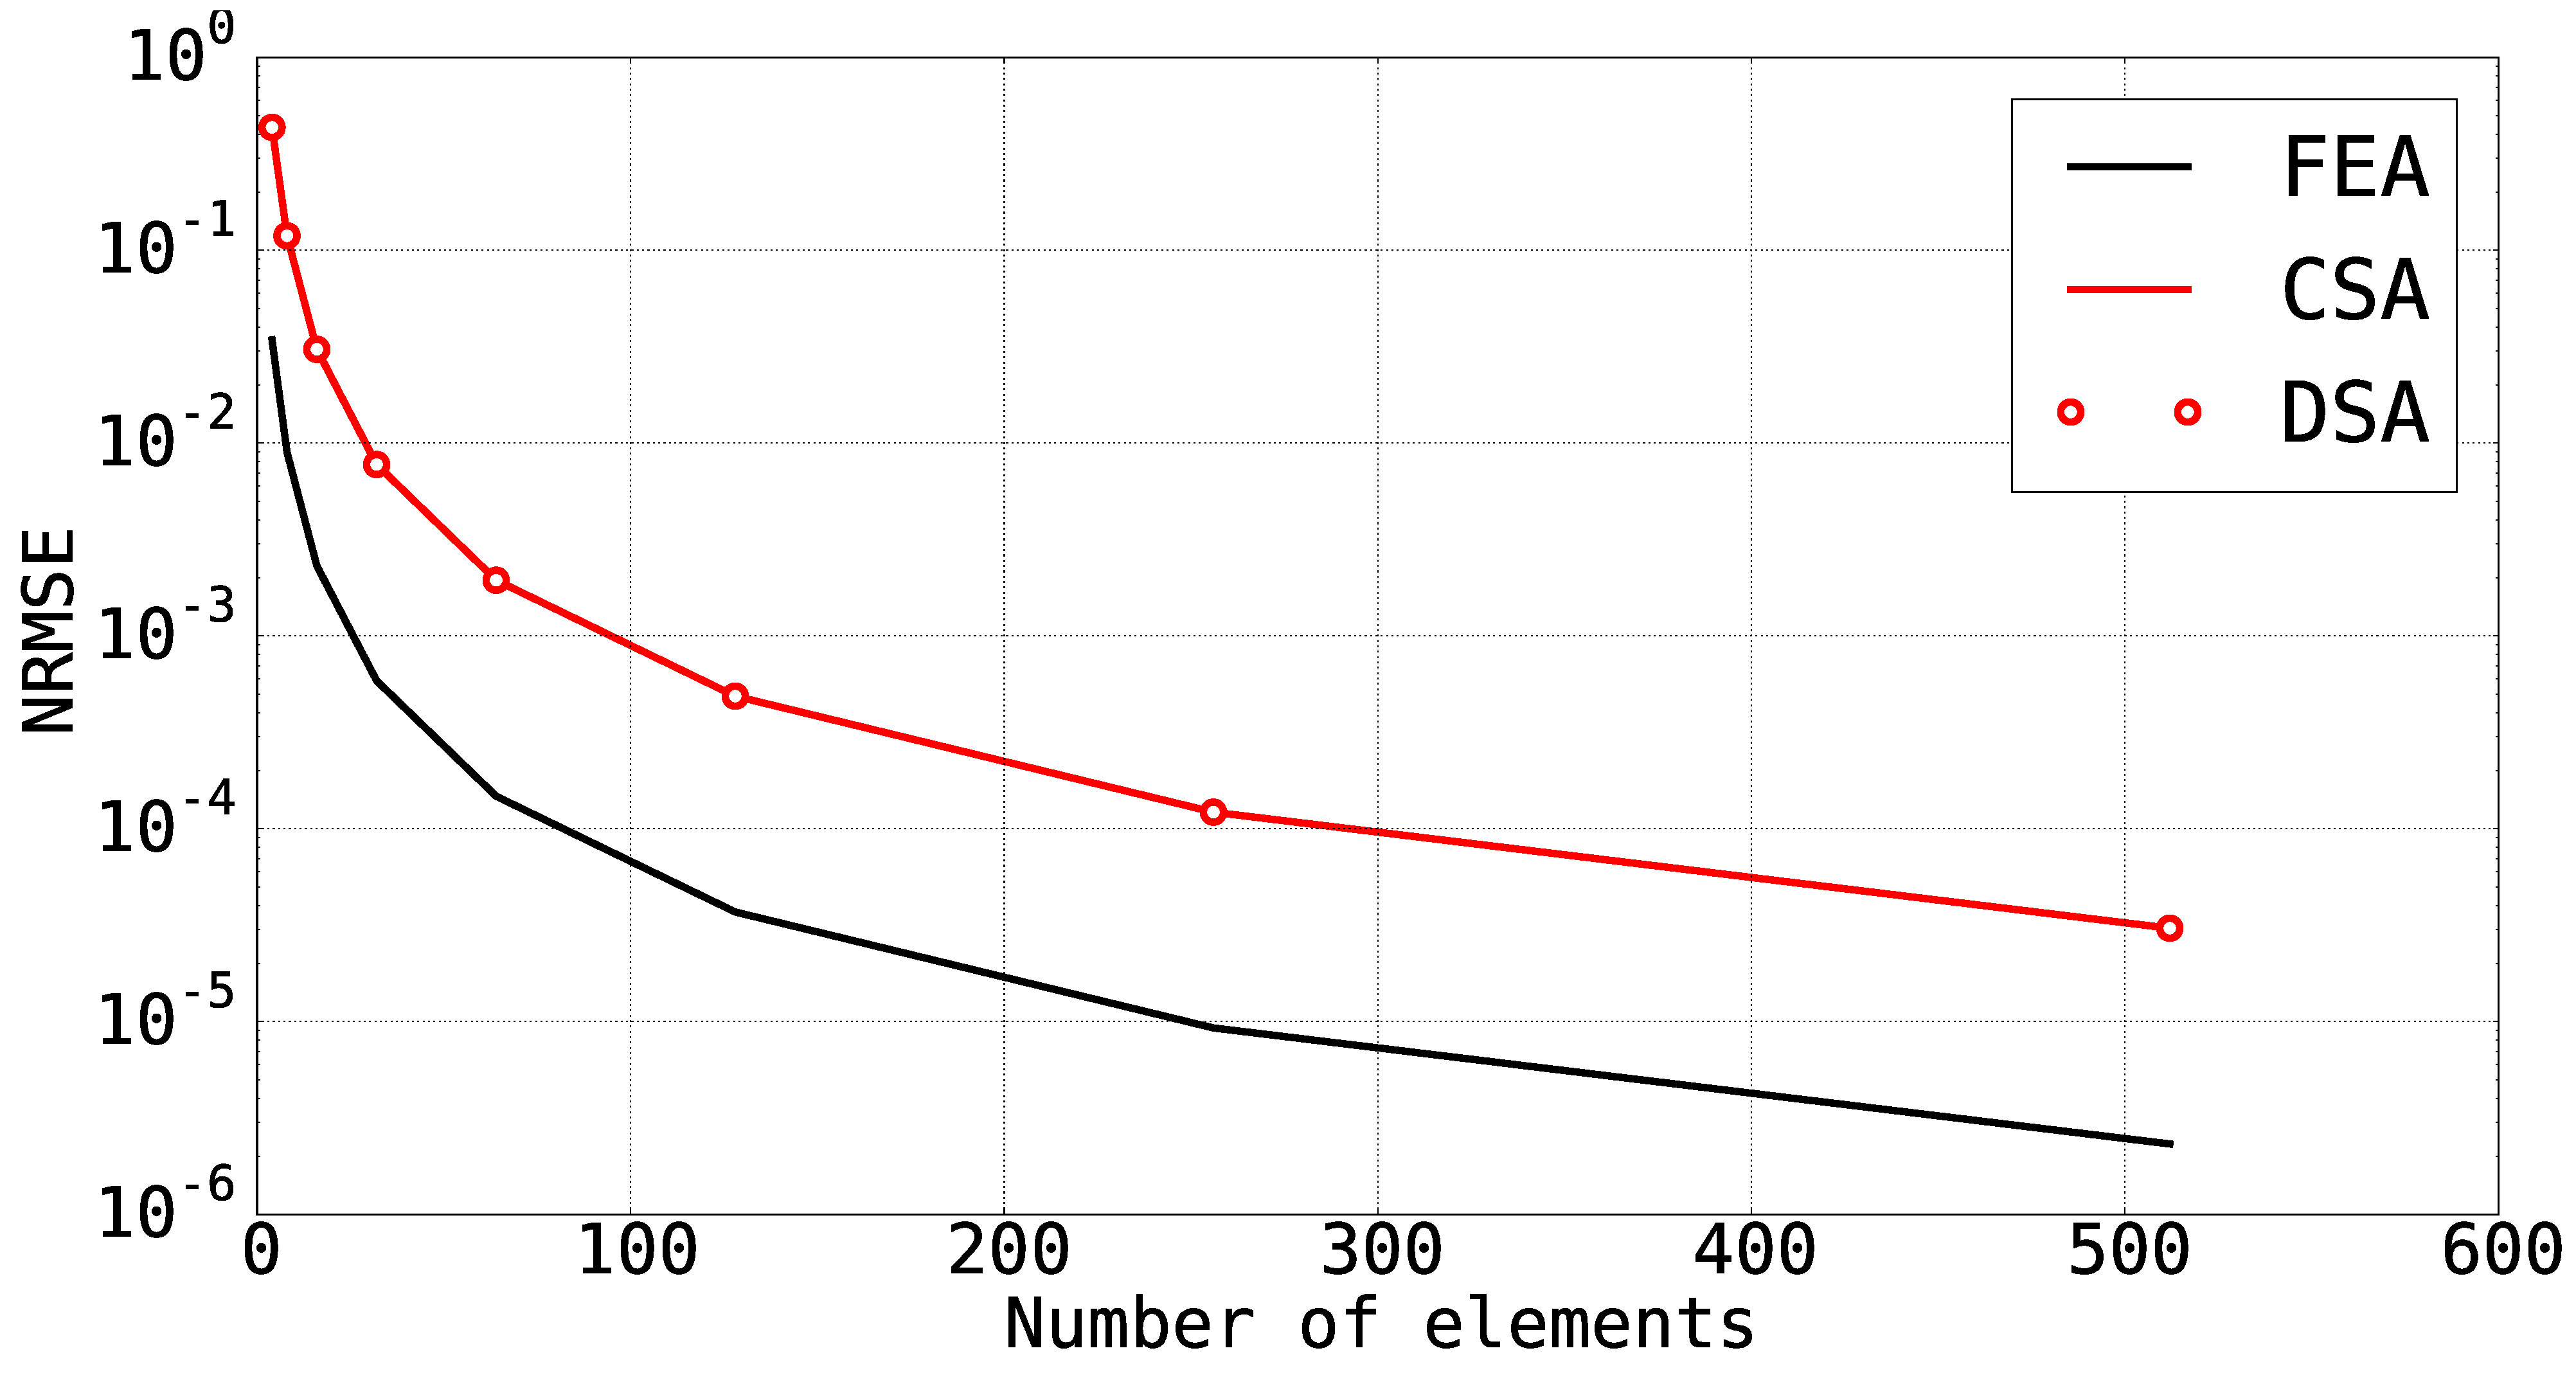
\includegraphics[width=14.00cm]{Chapter_2/figure/axial_bar_continuum_sensitivity_analysis.eps}
	\caption{Mesh convergence of the continuum (CSA) and discrete (DSA) sensitivity equations for axial bar problem. The results for the convergence of the analysis (FEA) also included in this graph.}
	\label{fig:C2_continuumSensitivityResults}
\end{figure}